\definecolor{zzttqq}{rgb}{0.15,0.35,0.15}

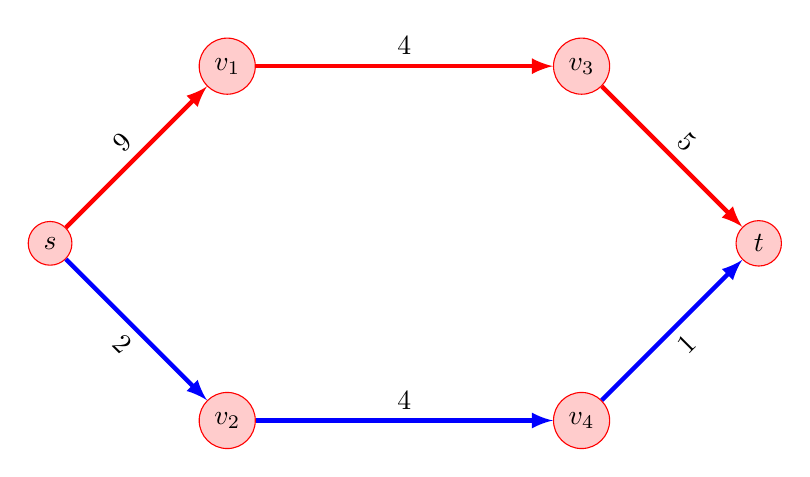
\begin{tikzpicture}[x=1.5cm, y=1.5cm]
	%\fill (-3.2,0) circle (0.1pt)node[anchor=east] {$20$};
	%\fill (3.2,0) circle (0.1pt)node[anchor=west] {$-20$};
    \node[circle,draw=red,fill=red!20!] (v1) at (-1.5,1.5) {$v_1$};
    \node[circle,draw=red,fill=red!20!] (v3) at (1.5,1.5) {$v_3$};
    \node[circle,draw=red,fill=red!20!] (t) at (3,0) {$t$};
    \node[circle,draw=red,fill=red!20!] (v4) at (1.5,-1.5) {$v_4$};
    \node[circle,draw=red,fill=red!20!] (v2) at (-1.5,-1.5) {$v_2$};
    \node[circle,draw=red,fill=red!20] (s) at (-3,0) {$s$};
    \draw[color=red, ultra thick, -latex]  (s) edge node[rotate = 45, above,color=black]{9} (v1);
	\draw[color=blue, ultra thick, -latex]  (s) edge node[rotate = -45, below,color=black]{2} (v2);
	\draw[-latex, color=red, ultra thick]  (v1) edge node[above,color=black]{4} (v3);
	\draw[-latex, color=blue, ultra thick]  (v2) edge node[above,color=black]{4} (v4);
	\draw[-latex, color=red, ultra thick]  (v3) edge node[rotate=-45,above,color=black]{5} (t);
	\draw[-latex, color=blue, ultra thick]  (v4) edge node[rotate=45,below,color=black]{1} (t);
\end{tikzpicture}